
% Default to the notebook output style

    


% Inherit from the specified cell style.




    
\documentclass[11pt]{article}

    
    
    \usepackage[T1]{fontenc}
    % Nicer default font (+ math font) than Computer Modern for most use cases
    \usepackage{mathpazo}

    % Basic figure setup, for now with no caption control since it's done
    % automatically by Pandoc (which extracts ![](path) syntax from Markdown).
    \usepackage{graphicx}
    % We will generate all images so they have a width \maxwidth. This means
    % that they will get their normal width if they fit onto the page, but
    % are scaled down if they would overflow the margins.
    \makeatletter
    \def\maxwidth{\ifdim\Gin@nat@width>\linewidth\linewidth
    \else\Gin@nat@width\fi}
    \makeatother
    \let\Oldincludegraphics\includegraphics
    % Set max figure width to be 80% of text width, for now hardcoded.
    \renewcommand{\includegraphics}[1]{\Oldincludegraphics[width=.8\maxwidth]{#1}}
    % Ensure that by default, figures have no caption (until we provide a
    % proper Figure object with a Caption API and a way to capture that
    % in the conversion process - todo).
    \usepackage{caption}
    \DeclareCaptionLabelFormat{nolabel}{}
    \captionsetup{labelformat=nolabel}

    \usepackage{adjustbox} % Used to constrain images to a maximum size 
    \usepackage{xcolor} % Allow colors to be defined
    \usepackage{enumerate} % Needed for markdown enumerations to work
    \usepackage{geometry} % Used to adjust the document margins
    \usepackage{amsmath} % Equations
    \usepackage{amssymb} % Equations
    \usepackage{textcomp} % defines textquotesingle
    % Hack from http://tex.stackexchange.com/a/47451/13684:
    \AtBeginDocument{%
        \def\PYZsq{\textquotesingle}% Upright quotes in Pygmentized code
    }
    \usepackage{upquote} % Upright quotes for verbatim code
    \usepackage{eurosym} % defines \euro
    \usepackage[mathletters]{ucs} % Extended unicode (utf-8) support
    \usepackage[utf8x]{inputenc} % Allow utf-8 characters in the tex document
    \usepackage{fancyvrb} % verbatim replacement that allows latex
    \usepackage{grffile} % extends the file name processing of package graphics 
                         % to support a larger range 
    % The hyperref package gives us a pdf with properly built
    % internal navigation ('pdf bookmarks' for the table of contents,
    % internal cross-reference links, web links for URLs, etc.)
    \usepackage{hyperref}
    \usepackage{longtable} % longtable support required by pandoc >1.10
    \usepackage{booktabs}  % table support for pandoc > 1.12.2
    \usepackage[inline]{enumitem} % IRkernel/repr support (it uses the enumerate* environment)
    \usepackage[normalem]{ulem} % ulem is needed to support strikethroughs (\sout)
                                % normalem makes italics be italics, not underlines
    

    
    
    % Colors for the hyperref package
    \definecolor{urlcolor}{rgb}{0,.145,.698}
    \definecolor{linkcolor}{rgb}{.71,0.21,0.01}
    \definecolor{citecolor}{rgb}{.12,.54,.11}

    % ANSI colors
    \definecolor{ansi-black}{HTML}{3E424D}
    \definecolor{ansi-black-intense}{HTML}{282C36}
    \definecolor{ansi-red}{HTML}{E75C58}
    \definecolor{ansi-red-intense}{HTML}{B22B31}
    \definecolor{ansi-green}{HTML}{00A250}
    \definecolor{ansi-green-intense}{HTML}{007427}
    \definecolor{ansi-yellow}{HTML}{DDB62B}
    \definecolor{ansi-yellow-intense}{HTML}{B27D12}
    \definecolor{ansi-blue}{HTML}{208FFB}
    \definecolor{ansi-blue-intense}{HTML}{0065CA}
    \definecolor{ansi-magenta}{HTML}{D160C4}
    \definecolor{ansi-magenta-intense}{HTML}{A03196}
    \definecolor{ansi-cyan}{HTML}{60C6C8}
    \definecolor{ansi-cyan-intense}{HTML}{258F8F}
    \definecolor{ansi-white}{HTML}{C5C1B4}
    \definecolor{ansi-white-intense}{HTML}{A1A6B2}

    % commands and environments needed by pandoc snippets
    % extracted from the output of `pandoc -s`
    \providecommand{\tightlist}{%
      \setlength{\itemsep}{0pt}\setlength{\parskip}{0pt}}
    \DefineVerbatimEnvironment{Highlighting}{Verbatim}{commandchars=\\\{\}}
    % Add ',fontsize=\small' for more characters per line
    \newenvironment{Shaded}{}{}
    \newcommand{\KeywordTok}[1]{\textcolor[rgb]{0.00,0.44,0.13}{\textbf{{#1}}}}
    \newcommand{\DataTypeTok}[1]{\textcolor[rgb]{0.56,0.13,0.00}{{#1}}}
    \newcommand{\DecValTok}[1]{\textcolor[rgb]{0.25,0.63,0.44}{{#1}}}
    \newcommand{\BaseNTok}[1]{\textcolor[rgb]{0.25,0.63,0.44}{{#1}}}
    \newcommand{\FloatTok}[1]{\textcolor[rgb]{0.25,0.63,0.44}{{#1}}}
    \newcommand{\CharTok}[1]{\textcolor[rgb]{0.25,0.44,0.63}{{#1}}}
    \newcommand{\StringTok}[1]{\textcolor[rgb]{0.25,0.44,0.63}{{#1}}}
    \newcommand{\CommentTok}[1]{\textcolor[rgb]{0.38,0.63,0.69}{\textit{{#1}}}}
    \newcommand{\OtherTok}[1]{\textcolor[rgb]{0.00,0.44,0.13}{{#1}}}
    \newcommand{\AlertTok}[1]{\textcolor[rgb]{1.00,0.00,0.00}{\textbf{{#1}}}}
    \newcommand{\FunctionTok}[1]{\textcolor[rgb]{0.02,0.16,0.49}{{#1}}}
    \newcommand{\RegionMarkerTok}[1]{{#1}}
    \newcommand{\ErrorTok}[1]{\textcolor[rgb]{1.00,0.00,0.00}{\textbf{{#1}}}}
    \newcommand{\NormalTok}[1]{{#1}}
    
    % Additional commands for more recent versions of Pandoc
    \newcommand{\ConstantTok}[1]{\textcolor[rgb]{0.53,0.00,0.00}{{#1}}}
    \newcommand{\SpecialCharTok}[1]{\textcolor[rgb]{0.25,0.44,0.63}{{#1}}}
    \newcommand{\VerbatimStringTok}[1]{\textcolor[rgb]{0.25,0.44,0.63}{{#1}}}
    \newcommand{\SpecialStringTok}[1]{\textcolor[rgb]{0.73,0.40,0.53}{{#1}}}
    \newcommand{\ImportTok}[1]{{#1}}
    \newcommand{\DocumentationTok}[1]{\textcolor[rgb]{0.73,0.13,0.13}{\textit{{#1}}}}
    \newcommand{\AnnotationTok}[1]{\textcolor[rgb]{0.38,0.63,0.69}{\textbf{\textit{{#1}}}}}
    \newcommand{\CommentVarTok}[1]{\textcolor[rgb]{0.38,0.63,0.69}{\textbf{\textit{{#1}}}}}
    \newcommand{\VariableTok}[1]{\textcolor[rgb]{0.10,0.09,0.49}{{#1}}}
    \newcommand{\ControlFlowTok}[1]{\textcolor[rgb]{0.00,0.44,0.13}{\textbf{{#1}}}}
    \newcommand{\OperatorTok}[1]{\textcolor[rgb]{0.40,0.40,0.40}{{#1}}}
    \newcommand{\BuiltInTok}[1]{{#1}}
    \newcommand{\ExtensionTok}[1]{{#1}}
    \newcommand{\PreprocessorTok}[1]{\textcolor[rgb]{0.74,0.48,0.00}{{#1}}}
    \newcommand{\AttributeTok}[1]{\textcolor[rgb]{0.49,0.56,0.16}{{#1}}}
    \newcommand{\InformationTok}[1]{\textcolor[rgb]{0.38,0.63,0.69}{\textbf{\textit{{#1}}}}}
    \newcommand{\WarningTok}[1]{\textcolor[rgb]{0.38,0.63,0.69}{\textbf{\textit{{#1}}}}}
    
    
    % Define a nice break command that doesn't care if a line doesn't already
    % exist.
    \def\br{\hspace*{\fill} \\* }
    % Math Jax compatability definitions
    \def\gt{>}
    \def\lt{<}
    % Document parameters
    \title{Ensembles}
    
    
    

    % Pygments definitions
    
\makeatletter
\def\PY@reset{\let\PY@it=\relax \let\PY@bf=\relax%
    \let\PY@ul=\relax \let\PY@tc=\relax%
    \let\PY@bc=\relax \let\PY@ff=\relax}
\def\PY@tok#1{\csname PY@tok@#1\endcsname}
\def\PY@toks#1+{\ifx\relax#1\empty\else%
    \PY@tok{#1}\expandafter\PY@toks\fi}
\def\PY@do#1{\PY@bc{\PY@tc{\PY@ul{%
    \PY@it{\PY@bf{\PY@ff{#1}}}}}}}
\def\PY#1#2{\PY@reset\PY@toks#1+\relax+\PY@do{#2}}

\expandafter\def\csname PY@tok@w\endcsname{\def\PY@tc##1{\textcolor[rgb]{0.73,0.73,0.73}{##1}}}
\expandafter\def\csname PY@tok@c\endcsname{\let\PY@it=\textit\def\PY@tc##1{\textcolor[rgb]{0.25,0.50,0.50}{##1}}}
\expandafter\def\csname PY@tok@cp\endcsname{\def\PY@tc##1{\textcolor[rgb]{0.74,0.48,0.00}{##1}}}
\expandafter\def\csname PY@tok@k\endcsname{\let\PY@bf=\textbf\def\PY@tc##1{\textcolor[rgb]{0.00,0.50,0.00}{##1}}}
\expandafter\def\csname PY@tok@kp\endcsname{\def\PY@tc##1{\textcolor[rgb]{0.00,0.50,0.00}{##1}}}
\expandafter\def\csname PY@tok@kt\endcsname{\def\PY@tc##1{\textcolor[rgb]{0.69,0.00,0.25}{##1}}}
\expandafter\def\csname PY@tok@o\endcsname{\def\PY@tc##1{\textcolor[rgb]{0.40,0.40,0.40}{##1}}}
\expandafter\def\csname PY@tok@ow\endcsname{\let\PY@bf=\textbf\def\PY@tc##1{\textcolor[rgb]{0.67,0.13,1.00}{##1}}}
\expandafter\def\csname PY@tok@nb\endcsname{\def\PY@tc##1{\textcolor[rgb]{0.00,0.50,0.00}{##1}}}
\expandafter\def\csname PY@tok@nf\endcsname{\def\PY@tc##1{\textcolor[rgb]{0.00,0.00,1.00}{##1}}}
\expandafter\def\csname PY@tok@nc\endcsname{\let\PY@bf=\textbf\def\PY@tc##1{\textcolor[rgb]{0.00,0.00,1.00}{##1}}}
\expandafter\def\csname PY@tok@nn\endcsname{\let\PY@bf=\textbf\def\PY@tc##1{\textcolor[rgb]{0.00,0.00,1.00}{##1}}}
\expandafter\def\csname PY@tok@ne\endcsname{\let\PY@bf=\textbf\def\PY@tc##1{\textcolor[rgb]{0.82,0.25,0.23}{##1}}}
\expandafter\def\csname PY@tok@nv\endcsname{\def\PY@tc##1{\textcolor[rgb]{0.10,0.09,0.49}{##1}}}
\expandafter\def\csname PY@tok@no\endcsname{\def\PY@tc##1{\textcolor[rgb]{0.53,0.00,0.00}{##1}}}
\expandafter\def\csname PY@tok@nl\endcsname{\def\PY@tc##1{\textcolor[rgb]{0.63,0.63,0.00}{##1}}}
\expandafter\def\csname PY@tok@ni\endcsname{\let\PY@bf=\textbf\def\PY@tc##1{\textcolor[rgb]{0.60,0.60,0.60}{##1}}}
\expandafter\def\csname PY@tok@na\endcsname{\def\PY@tc##1{\textcolor[rgb]{0.49,0.56,0.16}{##1}}}
\expandafter\def\csname PY@tok@nt\endcsname{\let\PY@bf=\textbf\def\PY@tc##1{\textcolor[rgb]{0.00,0.50,0.00}{##1}}}
\expandafter\def\csname PY@tok@nd\endcsname{\def\PY@tc##1{\textcolor[rgb]{0.67,0.13,1.00}{##1}}}
\expandafter\def\csname PY@tok@s\endcsname{\def\PY@tc##1{\textcolor[rgb]{0.73,0.13,0.13}{##1}}}
\expandafter\def\csname PY@tok@sd\endcsname{\let\PY@it=\textit\def\PY@tc##1{\textcolor[rgb]{0.73,0.13,0.13}{##1}}}
\expandafter\def\csname PY@tok@si\endcsname{\let\PY@bf=\textbf\def\PY@tc##1{\textcolor[rgb]{0.73,0.40,0.53}{##1}}}
\expandafter\def\csname PY@tok@se\endcsname{\let\PY@bf=\textbf\def\PY@tc##1{\textcolor[rgb]{0.73,0.40,0.13}{##1}}}
\expandafter\def\csname PY@tok@sr\endcsname{\def\PY@tc##1{\textcolor[rgb]{0.73,0.40,0.53}{##1}}}
\expandafter\def\csname PY@tok@ss\endcsname{\def\PY@tc##1{\textcolor[rgb]{0.10,0.09,0.49}{##1}}}
\expandafter\def\csname PY@tok@sx\endcsname{\def\PY@tc##1{\textcolor[rgb]{0.00,0.50,0.00}{##1}}}
\expandafter\def\csname PY@tok@m\endcsname{\def\PY@tc##1{\textcolor[rgb]{0.40,0.40,0.40}{##1}}}
\expandafter\def\csname PY@tok@gh\endcsname{\let\PY@bf=\textbf\def\PY@tc##1{\textcolor[rgb]{0.00,0.00,0.50}{##1}}}
\expandafter\def\csname PY@tok@gu\endcsname{\let\PY@bf=\textbf\def\PY@tc##1{\textcolor[rgb]{0.50,0.00,0.50}{##1}}}
\expandafter\def\csname PY@tok@gd\endcsname{\def\PY@tc##1{\textcolor[rgb]{0.63,0.00,0.00}{##1}}}
\expandafter\def\csname PY@tok@gi\endcsname{\def\PY@tc##1{\textcolor[rgb]{0.00,0.63,0.00}{##1}}}
\expandafter\def\csname PY@tok@gr\endcsname{\def\PY@tc##1{\textcolor[rgb]{1.00,0.00,0.00}{##1}}}
\expandafter\def\csname PY@tok@ge\endcsname{\let\PY@it=\textit}
\expandafter\def\csname PY@tok@gs\endcsname{\let\PY@bf=\textbf}
\expandafter\def\csname PY@tok@gp\endcsname{\let\PY@bf=\textbf\def\PY@tc##1{\textcolor[rgb]{0.00,0.00,0.50}{##1}}}
\expandafter\def\csname PY@tok@go\endcsname{\def\PY@tc##1{\textcolor[rgb]{0.53,0.53,0.53}{##1}}}
\expandafter\def\csname PY@tok@gt\endcsname{\def\PY@tc##1{\textcolor[rgb]{0.00,0.27,0.87}{##1}}}
\expandafter\def\csname PY@tok@err\endcsname{\def\PY@bc##1{\setlength{\fboxsep}{0pt}\fcolorbox[rgb]{1.00,0.00,0.00}{1,1,1}{\strut ##1}}}
\expandafter\def\csname PY@tok@kc\endcsname{\let\PY@bf=\textbf\def\PY@tc##1{\textcolor[rgb]{0.00,0.50,0.00}{##1}}}
\expandafter\def\csname PY@tok@kd\endcsname{\let\PY@bf=\textbf\def\PY@tc##1{\textcolor[rgb]{0.00,0.50,0.00}{##1}}}
\expandafter\def\csname PY@tok@kn\endcsname{\let\PY@bf=\textbf\def\PY@tc##1{\textcolor[rgb]{0.00,0.50,0.00}{##1}}}
\expandafter\def\csname PY@tok@kr\endcsname{\let\PY@bf=\textbf\def\PY@tc##1{\textcolor[rgb]{0.00,0.50,0.00}{##1}}}
\expandafter\def\csname PY@tok@bp\endcsname{\def\PY@tc##1{\textcolor[rgb]{0.00,0.50,0.00}{##1}}}
\expandafter\def\csname PY@tok@fm\endcsname{\def\PY@tc##1{\textcolor[rgb]{0.00,0.00,1.00}{##1}}}
\expandafter\def\csname PY@tok@vc\endcsname{\def\PY@tc##1{\textcolor[rgb]{0.10,0.09,0.49}{##1}}}
\expandafter\def\csname PY@tok@vg\endcsname{\def\PY@tc##1{\textcolor[rgb]{0.10,0.09,0.49}{##1}}}
\expandafter\def\csname PY@tok@vi\endcsname{\def\PY@tc##1{\textcolor[rgb]{0.10,0.09,0.49}{##1}}}
\expandafter\def\csname PY@tok@vm\endcsname{\def\PY@tc##1{\textcolor[rgb]{0.10,0.09,0.49}{##1}}}
\expandafter\def\csname PY@tok@sa\endcsname{\def\PY@tc##1{\textcolor[rgb]{0.73,0.13,0.13}{##1}}}
\expandafter\def\csname PY@tok@sb\endcsname{\def\PY@tc##1{\textcolor[rgb]{0.73,0.13,0.13}{##1}}}
\expandafter\def\csname PY@tok@sc\endcsname{\def\PY@tc##1{\textcolor[rgb]{0.73,0.13,0.13}{##1}}}
\expandafter\def\csname PY@tok@dl\endcsname{\def\PY@tc##1{\textcolor[rgb]{0.73,0.13,0.13}{##1}}}
\expandafter\def\csname PY@tok@s2\endcsname{\def\PY@tc##1{\textcolor[rgb]{0.73,0.13,0.13}{##1}}}
\expandafter\def\csname PY@tok@sh\endcsname{\def\PY@tc##1{\textcolor[rgb]{0.73,0.13,0.13}{##1}}}
\expandafter\def\csname PY@tok@s1\endcsname{\def\PY@tc##1{\textcolor[rgb]{0.73,0.13,0.13}{##1}}}
\expandafter\def\csname PY@tok@mb\endcsname{\def\PY@tc##1{\textcolor[rgb]{0.40,0.40,0.40}{##1}}}
\expandafter\def\csname PY@tok@mf\endcsname{\def\PY@tc##1{\textcolor[rgb]{0.40,0.40,0.40}{##1}}}
\expandafter\def\csname PY@tok@mh\endcsname{\def\PY@tc##1{\textcolor[rgb]{0.40,0.40,0.40}{##1}}}
\expandafter\def\csname PY@tok@mi\endcsname{\def\PY@tc##1{\textcolor[rgb]{0.40,0.40,0.40}{##1}}}
\expandafter\def\csname PY@tok@il\endcsname{\def\PY@tc##1{\textcolor[rgb]{0.40,0.40,0.40}{##1}}}
\expandafter\def\csname PY@tok@mo\endcsname{\def\PY@tc##1{\textcolor[rgb]{0.40,0.40,0.40}{##1}}}
\expandafter\def\csname PY@tok@ch\endcsname{\let\PY@it=\textit\def\PY@tc##1{\textcolor[rgb]{0.25,0.50,0.50}{##1}}}
\expandafter\def\csname PY@tok@cm\endcsname{\let\PY@it=\textit\def\PY@tc##1{\textcolor[rgb]{0.25,0.50,0.50}{##1}}}
\expandafter\def\csname PY@tok@cpf\endcsname{\let\PY@it=\textit\def\PY@tc##1{\textcolor[rgb]{0.25,0.50,0.50}{##1}}}
\expandafter\def\csname PY@tok@c1\endcsname{\let\PY@it=\textit\def\PY@tc##1{\textcolor[rgb]{0.25,0.50,0.50}{##1}}}
\expandafter\def\csname PY@tok@cs\endcsname{\let\PY@it=\textit\def\PY@tc##1{\textcolor[rgb]{0.25,0.50,0.50}{##1}}}

\def\PYZbs{\char`\\}
\def\PYZus{\char`\_}
\def\PYZob{\char`\{}
\def\PYZcb{\char`\}}
\def\PYZca{\char`\^}
\def\PYZam{\char`\&}
\def\PYZlt{\char`\<}
\def\PYZgt{\char`\>}
\def\PYZsh{\char`\#}
\def\PYZpc{\char`\%}
\def\PYZdl{\char`\$}
\def\PYZhy{\char`\-}
\def\PYZsq{\char`\'}
\def\PYZdq{\char`\"}
\def\PYZti{\char`\~}
% for compatibility with earlier versions
\def\PYZat{@}
\def\PYZlb{[}
\def\PYZrb{]}
\makeatother


    % Exact colors from NB
    \definecolor{incolor}{rgb}{0.0, 0.0, 0.5}
    \definecolor{outcolor}{rgb}{0.545, 0.0, 0.0}



    
    % Prevent overflowing lines due to hard-to-break entities
    \sloppy 
    % Setup hyperref package
    \hypersetup{
      breaklinks=true,  % so long urls are correctly broken across lines
      colorlinks=true,
      urlcolor=urlcolor,
      linkcolor=linkcolor,
      citecolor=citecolor,
      }
    % Slightly bigger margins than the latex defaults
    
    \geometry{verbose,tmargin=1in,bmargin=1in,lmargin=1in,rmargin=1in}
    
    

    \begin{document}
    
    
    \maketitle
    
    

    
    \hypertarget{fundamentos-em-data-science}{%
\section{Fundamentos em Data
Science}\label{fundamentos-em-data-science}}

\hypertarget{aula-5---algoritmos-de-ensemble}{%
\subsection{Aula 5 - Algoritmos de
Ensemble}\label{aula-5---algoritmos-de-ensemble}}

\begin{itemize}
\tightlist
\item
  Bagging
\item
  Boosting
\item
  Random Forests
\item
  AdaBoost
\item
  Stacking
\end{itemize}

Fábio Sato -
\href{mailto:fabiosato@gmail.com}{\nolinkurl{fabiosato@gmail.com}}

    \hypertarget{ensemble}{%
\section{Ensemble}\label{ensemble}}

Meta algoritmos que combinam várias técnicas de aprendizado de máquina
em um único modelo preditivo

Possibilita obter um desempenho preditivo melhor do que o obtido por um
modelo único

Objetivo: melhorar a predição de um modelo base (classificador ou
regressor)

    \hypertarget{ensemble}{%
\section{Ensemble}\label{ensemble}}

    \hypertarget{ensemble---tipos-de-muxe9todos}{%
\section{Ensemble - Tipos de
Métodos}\label{ensemble---tipos-de-muxe9todos}}

Os métodos de ensemble podem ser divididos em dois grupos principais:

\begin{itemize}
\tightlist
\item
  Sequencial
\item
  Paralelo
\end{itemize}

    \hypertarget{ensemble---muxe9todos-sequenciais}{%
\section{Ensemble - Métodos
Sequenciais}\label{ensemble---muxe9todos-sequenciais}}

Modelos base são gerados sequencialmente

Explora a \textbf{DEPENDÊNCIA} entre os modelos base

O desempenho global pode ser melhorado atribuindo pesos maiores a
exemplos classificados erroneamente pelo modelo anterior

    \hypertarget{ensemble---muxe9todos-paralelos}{%
\section{Ensemble - Métodos
Paralelos}\label{ensemble---muxe9todos-paralelos}}

Modelos base são gerados em paralelo

Explorar a \textbf{INDEPENDÊNCIA} entre os modelos base

Erros podem ser reduzidos drasticamente através da média

    \hypertarget{ensemble---homoguxeaneo-x-heteroguxeaneo}{%
\section{Ensemble - Homogêneo x
Heterogêneo}\label{ensemble---homoguxeaneo-x-heteroguxeaneo}}

\textbf{Homogêneo}: A maioria dos métodos de ensemble utilizam um
algoritmo base de aprendizado para produzir modelos do mesmo tipo

\textbf{Heterogêneo}: Existem alguns métodos que utilizam algoritmos
heterogêneos (de diferentes tipos)

Para que os métodos baseados em ensemble apresentem maior acurácia do
que qualquer um de seus membros individuais, os modelos de base devem
ser o mais precisos e \textbf{DIVERSOS} possíveis

    \hypertarget{ensemble---bagging}{%
\section{Ensemble - Bagging}\label{ensemble---bagging}}

Bagging: \emph{Boostrap Aggregation}

Redução da variância nas estimativas através da agregação (média) de
múltiplas estimativas

Treina algoritmos em diferentes subconjuntos de dados

As bases de treinamento para cada modelo base são geradas através de
amostragem aleatória com reposição

Para agregar as saídas dos modelos base, bagging utiliza o \textbf{voto}
para classificação e \textbf{média} para regressão

    \hypertarget{ensemble---bagging}{%
\section{Ensemble - Bagging}\label{ensemble---bagging}}

\[ f(x) = \frac{1}{M}\sum_{m=1}^{M}{f_{m}(x)} \]

    \hypertarget{ensemble---bagging-exemplo}{%
\section{Ensemble - Bagging: Exemplo}\label{ensemble---bagging-exemplo}}

    \begin{Verbatim}[commandchars=\\\{\}]
{\color{incolor}In [{\color{incolor}1}]:} \PY{o}{!}pip install mlxtend
\end{Verbatim}


    \begin{Verbatim}[commandchars=\\\{\}]
Requirement already satisfied (use --upgrade to upgrade): mlxtend in /Users/Sato/dev/treinamentos/fundamentos-data-science/env/lib/python3.6/site-packages
Requirement already satisfied (use --upgrade to upgrade): setuptools in /Users/Sato/dev/treinamentos/fundamentos-data-science/env/lib/python3.6/site-packages (from mlxtend)
\textcolor{ansi-yellow}{You are using pip version 7.1.2, however version 9.0.1 is available.
You should consider upgrading via the 'pip install --upgrade pip' command.}

    \end{Verbatim}

    \begin{Verbatim}[commandchars=\\\{\}]
{\color{incolor}In [{\color{incolor}2}]:} \PY{k+kn}{import} \PY{n+nn}{matplotlib} \PY{k}{as} \PY{n+nn}{mpl}
        
        \PY{n}{mpl}\PY{o}{.}\PY{n}{rcParams}\PY{p}{[}\PY{l+s+s1}{\PYZsq{}}\PY{l+s+s1}{figure.figsize}\PY{l+s+s1}{\PYZsq{}}\PY{p}{]} \PY{o}{=} \PY{p}{(}\PY{l+m+mi}{12}\PY{p}{,} \PY{l+m+mi}{8}\PY{p}{)}
\end{Verbatim}


    \begin{Verbatim}[commandchars=\\\{\}]
{\color{incolor}In [{\color{incolor}3}]:} \PY{k+kn}{import} \PY{n+nn}{itertools}
        \PY{k+kn}{import} \PY{n+nn}{numpy} \PY{k}{as} \PY{n+nn}{np}
        
        \PY{k+kn}{import} \PY{n+nn}{seaborn} \PY{k}{as} \PY{n+nn}{sns}
        \PY{k+kn}{import} \PY{n+nn}{matplotlib}\PY{n+nn}{.}\PY{n+nn}{pyplot} \PY{k}{as} \PY{n+nn}{plt}
        \PY{k+kn}{import} \PY{n+nn}{matplotlib}\PY{n+nn}{.}\PY{n+nn}{gridspec} \PY{k}{as} \PY{n+nn}{gridspec}
        
        \PY{k+kn}{from} \PY{n+nn}{sklearn} \PY{k}{import} \PY{n}{datasets}
        
        \PY{k+kn}{from} \PY{n+nn}{sklearn}\PY{n+nn}{.}\PY{n+nn}{tree} \PY{k}{import} \PY{n}{DecisionTreeClassifier}
        \PY{k+kn}{from} \PY{n+nn}{sklearn}\PY{n+nn}{.}\PY{n+nn}{neighbors} \PY{k}{import} \PY{n}{KNeighborsClassifier}
        \PY{k+kn}{from} \PY{n+nn}{sklearn}\PY{n+nn}{.}\PY{n+nn}{ensemble} \PY{k}{import} \PY{n}{BaggingClassifier}
        \PY{k+kn}{from} \PY{n+nn}{sklearn}\PY{n+nn}{.}\PY{n+nn}{model\PYZus{}selection} \PY{k}{import} \PY{n}{cross\PYZus{}val\PYZus{}score}\PY{p}{,} \PY{n}{train\PYZus{}test\PYZus{}split}
        
        \PY{k+kn}{from} \PY{n+nn}{mlxtend}\PY{n+nn}{.}\PY{n+nn}{plotting} \PY{k}{import} \PY{n}{plot\PYZus{}learning\PYZus{}curves}
        \PY{k+kn}{from} \PY{n+nn}{mlxtend}\PY{n+nn}{.}\PY{n+nn}{plotting} \PY{k}{import} \PY{n}{plot\PYZus{}decision\PYZus{}regions}
        
        \PY{n}{np}\PY{o}{.}\PY{n}{random}\PY{o}{.}\PY{n}{seed}\PY{p}{(}\PY{l+m+mi}{0}\PY{p}{)}
\end{Verbatim}


    \begin{Verbatim}[commandchars=\\\{\}]
{\color{incolor}In [{\color{incolor}4}]:} \PY{n}{iris} \PY{o}{=} \PY{n}{datasets}\PY{o}{.}\PY{n}{load\PYZus{}iris}\PY{p}{(}\PY{p}{)}
        \PY{n}{X}\PY{p}{,} \PY{n}{y} \PY{o}{=} \PY{n}{iris}\PY{o}{.}\PY{n}{data}\PY{p}{[}\PY{p}{:}\PY{p}{,} \PY{l+m+mi}{0}\PY{p}{:}\PY{l+m+mi}{2}\PY{p}{]}\PY{p}{,} \PY{n}{iris}\PY{o}{.}\PY{n}{target}
            
        \PY{n}{clf1} \PY{o}{=} \PY{n}{DecisionTreeClassifier}\PY{p}{(}\PY{n}{criterion}\PY{o}{=}\PY{l+s+s1}{\PYZsq{}}\PY{l+s+s1}{entropy}\PY{l+s+s1}{\PYZsq{}}\PY{p}{,} \PY{n}{max\PYZus{}depth}\PY{o}{=}\PY{l+m+mi}{3}\PY{p}{)}
        \PY{n}{clf2} \PY{o}{=} \PY{n}{KNeighborsClassifier}\PY{p}{(}\PY{n}{n\PYZus{}neighbors}\PY{o}{=}\PY{l+m+mi}{3}\PY{p}{)}    
        
        \PY{n}{bagging1} \PY{o}{=} \PY{n}{BaggingClassifier}\PY{p}{(}\PY{n}{base\PYZus{}estimator}\PY{o}{=}\PY{n}{clf1}\PY{p}{,} \PY{n}{n\PYZus{}estimators}\PY{o}{=}\PY{l+m+mi}{100}\PY{p}{,} 
                                     \PY{n}{max\PYZus{}samples}\PY{o}{=}\PY{l+m+mf}{0.3}\PY{p}{,} \PY{n}{max\PYZus{}features}\PY{o}{=}\PY{l+m+mf}{0.8}\PY{p}{)}
        
        \PY{n}{bagging2} \PY{o}{=} \PY{n}{BaggingClassifier}\PY{p}{(}\PY{n}{base\PYZus{}estimator}\PY{o}{=}\PY{n}{clf2}\PY{p}{,} \PY{n}{n\PYZus{}estimators}\PY{o}{=}\PY{l+m+mi}{100}\PY{p}{,} 
                                     \PY{n}{max\PYZus{}samples}\PY{o}{=}\PY{l+m+mf}{0.3}\PY{p}{,} \PY{n}{max\PYZus{}features}\PY{o}{=}\PY{l+m+mf}{0.8}\PY{p}{)}
\end{Verbatim}


    \begin{Verbatim}[commandchars=\\\{\}]
{\color{incolor}In [{\color{incolor}5}]:} \PY{n}{label} \PY{o}{=} \PY{p}{[}\PY{l+s+s1}{\PYZsq{}}\PY{l+s+s1}{Decision Tree}\PY{l+s+s1}{\PYZsq{}}\PY{p}{,} \PY{l+s+s1}{\PYZsq{}}\PY{l+s+s1}{k\PYZhy{}NN}\PY{l+s+s1}{\PYZsq{}}\PY{p}{,} \PY{l+s+s1}{\PYZsq{}}\PY{l+s+s1}{Bagging Tree}\PY{l+s+s1}{\PYZsq{}}\PY{p}{,} \PY{l+s+s1}{\PYZsq{}}\PY{l+s+s1}{Bagging k\PYZhy{}NN}\PY{l+s+s1}{\PYZsq{}}\PY{p}{]}
        \PY{n}{clf\PYZus{}list} \PY{o}{=} \PY{p}{[}\PY{n}{clf1}\PY{p}{,} \PY{n}{clf2}\PY{p}{,} \PY{n}{bagging1}\PY{p}{,} \PY{n}{bagging2}\PY{p}{]}
        
        \PY{n}{fig} \PY{o}{=} \PY{n}{plt}\PY{o}{.}\PY{n}{figure}\PY{p}{(}\PY{n}{figsize}\PY{o}{=}\PY{p}{(}\PY{l+m+mi}{10}\PY{p}{,} \PY{l+m+mi}{8}\PY{p}{)}\PY{p}{)}
        \PY{n}{gs} \PY{o}{=} \PY{n}{gridspec}\PY{o}{.}\PY{n}{GridSpec}\PY{p}{(}\PY{l+m+mi}{2}\PY{p}{,} \PY{l+m+mi}{2}\PY{p}{)}
        \PY{n}{grid} \PY{o}{=} \PY{n}{itertools}\PY{o}{.}\PY{n}{product}\PY{p}{(}\PY{p}{[}\PY{l+m+mi}{0}\PY{p}{,}\PY{l+m+mi}{1}\PY{p}{]}\PY{p}{,}\PY{n}{repeat}\PY{o}{=}\PY{l+m+mi}{2}\PY{p}{)}
        
        \PY{k}{for} \PY{n}{clf}\PY{p}{,} \PY{n}{label}\PY{p}{,} \PY{n}{grd} \PY{o+ow}{in} \PY{n+nb}{zip}\PY{p}{(}\PY{n}{clf\PYZus{}list}\PY{p}{,} \PY{n}{label}\PY{p}{,} \PY{n}{grid}\PY{p}{)}\PY{p}{:}        
            \PY{n}{scores} \PY{o}{=} \PY{n}{cross\PYZus{}val\PYZus{}score}\PY{p}{(}\PY{n}{clf}\PY{p}{,} \PY{n}{X}\PY{p}{,} \PY{n}{y}\PY{p}{,} \PY{n}{cv}\PY{o}{=}\PY{l+m+mi}{3}\PY{p}{,} \PY{n}{scoring}\PY{o}{=}\PY{l+s+s1}{\PYZsq{}}\PY{l+s+s1}{accuracy}\PY{l+s+s1}{\PYZsq{}}\PY{p}{)}
            \PY{n+nb}{print}\PY{p}{(}\PY{l+s+s2}{\PYZdq{}}\PY{l+s+s2}{Accuracy: }\PY{l+s+si}{\PYZpc{}.2f}\PY{l+s+s2}{ (+/\PYZhy{} }\PY{l+s+si}{\PYZpc{}.2f}\PY{l+s+s2}{) [}\PY{l+s+si}{\PYZpc{}s}\PY{l+s+s2}{]}\PY{l+s+s2}{\PYZdq{}} \PY{o}{\PYZpc{}}\PY{p}{(}\PY{n}{scores}\PY{o}{.}\PY{n}{mean}\PY{p}{(}\PY{p}{)}\PY{p}{,} \PY{n}{scores}\PY{o}{.}\PY{n}{std}\PY{p}{(}\PY{p}{)}\PY{p}{,} \PY{n}{label}\PY{p}{)}\PY{p}{)}
                
            \PY{n}{clf}\PY{o}{.}\PY{n}{fit}\PY{p}{(}\PY{n}{X}\PY{p}{,} \PY{n}{y}\PY{p}{)}
            \PY{n}{ax} \PY{o}{=} \PY{n}{plt}\PY{o}{.}\PY{n}{subplot}\PY{p}{(}\PY{n}{gs}\PY{p}{[}\PY{n}{grd}\PY{p}{[}\PY{l+m+mi}{0}\PY{p}{]}\PY{p}{,} \PY{n}{grd}\PY{p}{[}\PY{l+m+mi}{1}\PY{p}{]}\PY{p}{]}\PY{p}{)}
            \PY{n}{fig} \PY{o}{=} \PY{n}{plot\PYZus{}decision\PYZus{}regions}\PY{p}{(}\PY{n}{X}\PY{o}{=}\PY{n}{X}\PY{p}{,} \PY{n}{y}\PY{o}{=}\PY{n}{y}\PY{p}{,} \PY{n}{clf}\PY{o}{=}\PY{n}{clf}\PY{p}{,} \PY{n}{legend}\PY{o}{=}\PY{l+m+mi}{2}\PY{p}{)}
            \PY{n}{plt}\PY{o}{.}\PY{n}{title}\PY{p}{(}\PY{n}{label}\PY{p}{)}
\end{Verbatim}


    \begin{Verbatim}[commandchars=\\\{\}]
Accuracy: 0.67 (+/- 0.03) [Decision Tree]
Accuracy: 0.73 (+/- 0.03) [k-NN]
Accuracy: 0.73 (+/- 0.04) [Bagging Tree]
Accuracy: 0.76 (+/- 0.06) [Bagging k-NN]

    \end{Verbatim}

    \begin{Verbatim}[commandchars=\\\{\}]
{\color{incolor}In [{\color{incolor}6}]:} \PY{n}{plt}\PY{o}{.}\PY{n}{show}\PY{p}{(}\PY{p}{)}
\end{Verbatim}


    \begin{center}
    \adjustimage{max size={0.9\linewidth}{0.9\paperheight}}{output_15_0.png}
    \end{center}
    { \hspace*{\fill} \\}
    
    \hypertarget{random-forests}{%
\section{Random Forests}\label{random-forests}}

Um exemplo bem comum de classe de algoritmo de ensemble são as florestas
aleatórias de árvores (Random Forests)

Em Random Forests, cada árvore é um ensemble construído a partir de uma
amostra com substituição.

Além disso, ao invés de utilizar todas as características, um conjunto
aleatório de características é selecionado tornando o processo de
criação de árvores ainda mais aleatório.

Como resultado, o viés da floresta cresce ligeiramente mas a variância
diminui significativamente resultando em um modelo muito melhor.

    \hypertarget{random-forests}{%
\section{Random Forests}\label{random-forests}}

\begin{figure}
\centering
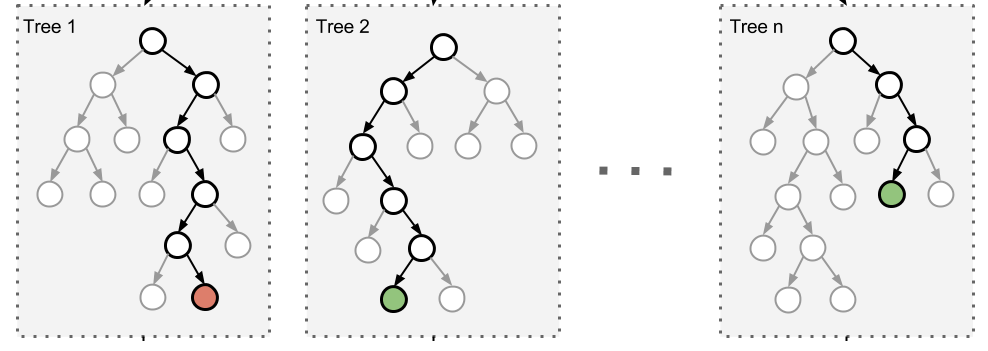
\includegraphics{figuras/random-forests.png}
\caption{Random Forests}
\end{figure}

    \hypertarget{random-forests---exercuxedcio}{%
\section{Random Forests -
Exercício}\label{random-forests---exercuxedcio}}

Implemente um modelo baseado em Random Forests para a base de dados
`Boston House Prices'

    

    \begin{Verbatim}[commandchars=\\\{\}]
{\color{incolor}In [{\color{incolor}7}]:} \PY{k+kn}{from} \PY{n+nn}{sklearn}\PY{n+nn}{.}\PY{n+nn}{datasets} \PY{k}{import} \PY{n}{load\PYZus{}boston}
        \PY{k+kn}{from} \PY{n+nn}{sklearn}\PY{n+nn}{.}\PY{n+nn}{ensemble} \PY{k}{import} \PY{n}{RandomForestRegressor}
\end{Verbatim}


    \begin{Verbatim}[commandchars=\\\{\}]
{\color{incolor}In [{\color{incolor}8}]:} \PY{n}{boston} \PY{o}{=} \PY{n}{load\PYZus{}boston}\PY{p}{(}\PY{p}{)}
        \PY{n+nb}{dir}\PY{p}{(}\PY{n}{boston}\PY{p}{)}
\end{Verbatim}


\begin{Verbatim}[commandchars=\\\{\}]
{\color{outcolor}Out[{\color{outcolor}8}]:} ['DESCR', 'data', 'feature\_names', 'target']
\end{Verbatim}
            
    \begin{Verbatim}[commandchars=\\\{\}]
{\color{incolor}In [{\color{incolor}9}]:} \PY{k+kn}{import} \PY{n+nn}{pandas} \PY{k}{as} \PY{n+nn}{pd}
\end{Verbatim}


    \begin{Verbatim}[commandchars=\\\{\}]
{\color{incolor}In [{\color{incolor}10}]:} \PY{n}{df} \PY{o}{=} \PY{n}{pd}\PY{o}{.}\PY{n}{DataFrame}\PY{p}{(}\PY{n}{boston}\PY{o}{.}\PY{n}{data}\PY{p}{,} \PY{n}{columns}\PY{o}{=}\PY{n}{boston}\PY{o}{.}\PY{n}{feature\PYZus{}names}\PY{p}{)}
         \PY{n}{df}\PY{p}{[}\PY{l+s+s1}{\PYZsq{}}\PY{l+s+s1}{PRICE}\PY{l+s+s1}{\PYZsq{}}\PY{p}{]} \PY{o}{=} \PY{n}{boston}\PY{o}{.}\PY{n}{target}
\end{Verbatim}


    \begin{Verbatim}[commandchars=\\\{\}]
{\color{incolor}In [{\color{incolor}11}]:} \PY{n}{df}\PY{o}{.}\PY{n}{describe}\PY{p}{(}\PY{p}{)}
\end{Verbatim}


\begin{Verbatim}[commandchars=\\\{\}]
{\color{outcolor}Out[{\color{outcolor}11}]:}              CRIM          ZN       INDUS        CHAS         NOX          RM  \textbackslash{}
         count  506.000000  506.000000  506.000000  506.000000  506.000000  506.000000   
         mean     3.593761   11.363636   11.136779    0.069170    0.554695    6.284634   
         std      8.596783   23.322453    6.860353    0.253994    0.115878    0.702617   
         min      0.006320    0.000000    0.460000    0.000000    0.385000    3.561000   
         25\%      0.082045    0.000000    5.190000    0.000000    0.449000    5.885500   
         50\%      0.256510    0.000000    9.690000    0.000000    0.538000    6.208500   
         75\%      3.647423   12.500000   18.100000    0.000000    0.624000    6.623500   
         max     88.976200  100.000000   27.740000    1.000000    0.871000    8.780000   
         
                       AGE         DIS         RAD         TAX     PTRATIO           B  \textbackslash{}
         count  506.000000  506.000000  506.000000  506.000000  506.000000  506.000000   
         mean    68.574901    3.795043    9.549407  408.237154   18.455534  356.674032   
         std     28.148861    2.105710    8.707259  168.537116    2.164946   91.294864   
         min      2.900000    1.129600    1.000000  187.000000   12.600000    0.320000   
         25\%     45.025000    2.100175    4.000000  279.000000   17.400000  375.377500   
         50\%     77.500000    3.207450    5.000000  330.000000   19.050000  391.440000   
         75\%     94.075000    5.188425   24.000000  666.000000   20.200000  396.225000   
         max    100.000000   12.126500   24.000000  711.000000   22.000000  396.900000   
         
                     LSTAT       PRICE  
         count  506.000000  506.000000  
         mean    12.653063   22.532806  
         std      7.141062    9.197104  
         min      1.730000    5.000000  
         25\%      6.950000   17.025000  
         50\%     11.360000   21.200000  
         75\%     16.955000   25.000000  
         max     37.970000   50.000000  
\end{Verbatim}
            
    \begin{Verbatim}[commandchars=\\\{\}]
{\color{incolor}In [{\color{incolor}12}]:} \PY{n}{rf} \PY{o}{=} \PY{n}{RandomForestRegressor}\PY{p}{(}\PY{n}{max\PYZus{}depth}\PY{o}{=}\PY{l+m+mi}{10}\PY{p}{,} \PY{n}{n\PYZus{}estimators}\PY{o}{=}\PY{l+m+mi}{10}\PY{p}{)}
         \PY{n}{rf}\PY{o}{.}\PY{n}{fit}\PY{p}{(}\PY{n}{boston}\PY{o}{.}\PY{n}{data}\PY{p}{,} \PY{n}{boston}\PY{o}{.}\PY{n}{target}\PY{p}{)}
\end{Verbatim}


\begin{Verbatim}[commandchars=\\\{\}]
{\color{outcolor}Out[{\color{outcolor}12}]:} RandomForestRegressor(bootstrap=True, criterion='mse', max\_depth=10,
                    max\_features='auto', max\_leaf\_nodes=None,
                    min\_impurity\_decrease=0.0, min\_impurity\_split=None,
                    min\_samples\_leaf=1, min\_samples\_split=2,
                    min\_weight\_fraction\_leaf=0.0, n\_estimators=10, n\_jobs=1,
                    oob\_score=False, random\_state=None, verbose=0, warm\_start=False)
\end{Verbatim}
            
    \begin{Verbatim}[commandchars=\\\{\}]
{\color{incolor}In [{\color{incolor}13}]:} \PY{n}{y\PYZus{}pred} \PY{o}{=} \PY{n}{rf}\PY{o}{.}\PY{n}{predict}\PY{p}{(}\PY{n}{boston}\PY{o}{.}\PY{n}{data}\PY{p}{)}
\end{Verbatim}


    \begin{Verbatim}[commandchars=\\\{\}]
{\color{incolor}In [{\color{incolor}14}]:} \PY{n}{plt}\PY{o}{.}\PY{n}{scatter}\PY{p}{(}\PY{n}{boston}\PY{o}{.}\PY{n}{target}\PY{p}{,} \PY{n}{y\PYZus{}pred}\PY{p}{)}
         \PY{n}{plt}\PY{o}{.}\PY{n}{show}\PY{p}{(}\PY{p}{)}
\end{Verbatim}


    \begin{center}
    \adjustimage{max size={0.9\linewidth}{0.9\paperheight}}{output_27_0.png}
    \end{center}
    { \hspace*{\fill} \\}
    
    \begin{Verbatim}[commandchars=\\\{\}]
{\color{incolor}In [{\color{incolor}15}]:} \PY{k+kn}{from} \PY{n+nn}{sklearn}\PY{n+nn}{.}\PY{n+nn}{metrics} \PY{k}{import} \PY{n}{mean\PYZus{}squared\PYZus{}error}\PY{p}{,} \PY{n}{r2\PYZus{}score}
         
         \PY{n+nb}{print}\PY{p}{(}\PY{l+s+s1}{\PYZsq{}}\PY{l+s+si}{\PYZpc{}.2f}\PY{l+s+s1}{\PYZsq{}} \PY{o}{\PYZpc{}} \PY{n}{mean\PYZus{}squared\PYZus{}error}\PY{p}{(}\PY{n}{boston}\PY{o}{.}\PY{n}{target}\PY{p}{,} \PY{n}{y\PYZus{}pred}\PY{p}{)}\PY{p}{)}
         \PY{n+nb}{print}\PY{p}{(}\PY{l+s+s1}{\PYZsq{}}\PY{l+s+si}{\PYZpc{}.2f}\PY{l+s+s1}{\PYZsq{}} \PY{o}{\PYZpc{}} \PY{n}{r2\PYZus{}score}\PY{p}{(}\PY{n}{boston}\PY{o}{.}\PY{n}{target}\PY{p}{,} \PY{n}{y\PYZus{}pred}\PY{p}{)}\PY{p}{)}
\end{Verbatim}


    \begin{Verbatim}[commandchars=\\\{\}]
2.24
0.97

    \end{Verbatim}

    \begin{Verbatim}[commandchars=\\\{\}]
{\color{incolor}In [{\color{incolor}16}]:} \PY{k+kn}{import} \PY{n+nn}{numpy} \PY{k}{as} \PY{n+nn}{np}
         
         \PY{n}{importances} \PY{o}{=} \PY{n}{rf}\PY{o}{.}\PY{n}{feature\PYZus{}importances\PYZus{}}
         
         \PY{n+nb}{print}\PY{p}{(}\PY{n}{importances}\PY{p}{)}
         \PY{n}{plt}\PY{o}{.}\PY{n}{bar}\PY{p}{(}\PY{n+nb}{range}\PY{p}{(}\PY{n+nb}{len}\PY{p}{(}\PY{n}{boston}\PY{o}{.}\PY{n}{feature\PYZus{}names}\PY{p}{)}\PY{p}{)}\PY{p}{,} \PY{n}{importances}\PY{p}{)}
         \PY{n}{plt}\PY{o}{.}\PY{n}{show}\PY{p}{(}\PY{p}{)}
\end{Verbatim}


    \begin{Verbatim}[commandchars=\\\{\}]
[  3.21677097e-02   8.41340782e-04   8.96121378e-03   2.11566867e-04
   2.31108909e-02   4.75535099e-01   1.13174231e-02   6.25328370e-02
   3.54499657e-03   1.43623266e-02   1.43355808e-02   1.53191041e-02
   3.37759911e-01]

    \end{Verbatim}

    \begin{center}
    \adjustimage{max size={0.9\linewidth}{0.9\paperheight}}{output_29_1.png}
    \end{center}
    { \hspace*{\fill} \\}
    
    \hypertarget{ensemble---boosting}{%
\section{Ensemble - Boosting}\label{ensemble---boosting}}

Família de algoritmos que convertem classificadores fracos em algoritmos
de aprendizado fortes.

Princípio fundamental: treinar uma sequência de classificadores fracos
que são apenas um pouco melhores que adivinhar aleatoriamente (ex:
pequenas árvores de decisão).

    \hypertarget{ensemble---boosting}{%
\section{Ensemble - Boosting}\label{ensemble---boosting}}

Os classificadores fracos são treinados em versões com peso ponderado
dos dados. Mais peso é atribuído aos exemplos que foram classificadores
errôneamente pelo modelo anterior.

As previsões são combinadas usando voto ponderado (classificação) ou
soma ponderada (regressão) para produzir a estimativa final.

    \hypertarget{boosting---adaboost}{%
\section{Boosting - AdaBoost}\label{boosting---adaboost}}

Os classificadores fracos no AdaBoost são árvores de decisão com
profundida igual a 1, chamados de \emph{stumps} (tocos).

O AdaBoost pondera as observações, colocando mais peso na dificuldade de
classificar exemplos e menos naqueles que já são classificados
corretamente.

Novos classificadores fracos são adicionados sequencialmente e focam seu
treinamento nos padrões mais difíceis.

Exemplos que são difíceis de serem classificados recebem cada vez mais
peso até que o algoritmo os classifiquem corretamente.

    \hypertarget{boosting-adaboost}{%
\section{Boosting: AdaBoost}\label{boosting-adaboost}}

\begin{enumerate}
\def\labelenumi{\arabic{enumi}.}
\tightlist
\item
  Atribua pesos uniformes ao vetor \(w\) onde \$ \sum\_\{i\} \{w\_i\} =
  1 \$
\item
  Para cada \(j\) em \(m\) rodadas de boosting, faça:
\item
  Treine um classificador fraco:
  \(c_j = train(\mathbf{X}, \mathbf{y}, \mathbf{w})\)
\item
  Estime as novas classes:
  \(\mathbf{\widehat{y}} = predict(C_j, \mathbf{X})\)
\item
  Calcule a taxa de erro ponderado: \$ \epsilon = \mathbf{w}
  \cdot (\mathbf{\widehat{y}} == \mathbf{y})\$
\item
  Calcule o coeficiente:
  \(\alpha_{j} = 0.5 log \frac{1 - \epsilon}{\epsilon}\)
\item
  Atualize os pesos: \$ \mathbf{w} = \mathbf{w} \times exp(-\alpha\_j
  \times \mathbf{\widehat{y}} \times \mathbf{y}) \$
\item
  Normalize os pesos para que a soma seja 1: \$ \mathbf{w} := \mathbf{w}
  / \sum\_i \{w\_i\}\$
\item
  Realize as estimativas finais: \$ \mathbf{\widehat{y}} =
  (\sum\_\{j=1\}\^{}\{m\}\{(\alpha\_j \times predict(C\_j,
  \mathbf{X}\})) \textgreater{} 0)\$
\end{enumerate}

Onde: \$ (\mathbf{\hat{y}} == \mathbf{y}) \$ no passo 5 se refere a
vetores contendo 0s ou 1s, onde 1 é atribuído para estimativas corretas
e 0 para erradas

    \hypertarget{boosting-exemplo}{%
\section{Boosting: Exemplo}\label{boosting-exemplo}}

    \begin{Verbatim}[commandchars=\\\{\}]
{\color{incolor}In [{\color{incolor}17}]:} \PY{k+kn}{import} \PY{n+nn}{itertools}
         \PY{k+kn}{import} \PY{n+nn}{numpy} \PY{k}{as} \PY{n+nn}{np}
         
         \PY{k+kn}{import} \PY{n+nn}{seaborn} \PY{k}{as} \PY{n+nn}{sns}
         \PY{k+kn}{import} \PY{n+nn}{matplotlib}\PY{n+nn}{.}\PY{n+nn}{pyplot} \PY{k}{as} \PY{n+nn}{plt}
         \PY{k+kn}{import} \PY{n+nn}{matplotlib}\PY{n+nn}{.}\PY{n+nn}{gridspec} \PY{k}{as} \PY{n+nn}{gridspec}
         
         \PY{k+kn}{from} \PY{n+nn}{sklearn} \PY{k}{import} \PY{n}{datasets}
         
         \PY{k+kn}{from} \PY{n+nn}{sklearn}\PY{n+nn}{.}\PY{n+nn}{ensemble} \PY{k}{import} \PY{n}{AdaBoostClassifier}
         \PY{k+kn}{from} \PY{n+nn}{sklearn}\PY{n+nn}{.}\PY{n+nn}{model\PYZus{}selection} \PY{k}{import} \PY{n}{cross\PYZus{}val\PYZus{}score}\PY{p}{,} \PY{n}{train\PYZus{}test\PYZus{}split}
         
         \PY{k+kn}{from} \PY{n+nn}{mlxtend}\PY{n+nn}{.}\PY{n+nn}{plotting} \PY{k}{import} \PY{n}{plot\PYZus{}learning\PYZus{}curves}
         \PY{k+kn}{from} \PY{n+nn}{mlxtend}\PY{n+nn}{.}\PY{n+nn}{plotting} \PY{k}{import} \PY{n}{plot\PYZus{}decision\PYZus{}regions}
\end{Verbatim}


    \begin{Verbatim}[commandchars=\\\{\}]
{\color{incolor}In [{\color{incolor}18}]:} \PY{n}{iris} \PY{o}{=} \PY{n}{datasets}\PY{o}{.}\PY{n}{load\PYZus{}iris}\PY{p}{(}\PY{p}{)}
         \PY{n}{X}\PY{p}{,} \PY{n}{y} \PY{o}{=} \PY{n}{iris}\PY{o}{.}\PY{n}{data}\PY{p}{[}\PY{p}{:}\PY{p}{,} \PY{l+m+mi}{0}\PY{p}{:}\PY{l+m+mi}{2}\PY{p}{]}\PY{p}{,} \PY{n}{iris}\PY{o}{.}\PY{n}{target}
             
         \PY{n}{clf} \PY{o}{=} \PY{n}{DecisionTreeClassifier}\PY{p}{(}\PY{n}{criterion}\PY{o}{=}\PY{l+s+s1}{\PYZsq{}}\PY{l+s+s1}{entropy}\PY{l+s+s1}{\PYZsq{}}\PY{p}{,} \PY{n}{max\PYZus{}depth}\PY{o}{=}\PY{l+m+mi}{1}\PY{p}{)}
         
         \PY{n}{num\PYZus{}est} \PY{o}{=} \PY{p}{[}\PY{l+m+mi}{1}\PY{p}{,} \PY{l+m+mi}{2}\PY{p}{,} \PY{l+m+mi}{3}\PY{p}{,} \PY{l+m+mi}{6}\PY{p}{]}
         \PY{n}{label} \PY{o}{=} \PY{p}{[}\PY{l+s+s1}{\PYZsq{}}\PY{l+s+s1}{AdaBoost (n=1)}\PY{l+s+s1}{\PYZsq{}}\PY{p}{,} \PY{l+s+s1}{\PYZsq{}}\PY{l+s+s1}{AdaBoost (n=2)}\PY{l+s+s1}{\PYZsq{}}\PY{p}{,} \PY{l+s+s1}{\PYZsq{}}\PY{l+s+s1}{AdaBoost (n=3)}\PY{l+s+s1}{\PYZsq{}}\PY{p}{,} 
                  \PY{l+s+s1}{\PYZsq{}}\PY{l+s+s1}{AdaBoost (n=10)}\PY{l+s+s1}{\PYZsq{}}\PY{p}{]}
\end{Verbatim}


    \begin{Verbatim}[commandchars=\\\{\}]
{\color{incolor}In [{\color{incolor}19}]:} \PY{n}{fig} \PY{o}{=} \PY{n}{plt}\PY{o}{.}\PY{n}{figure}\PY{p}{(}\PY{n}{figsize}\PY{o}{=}\PY{p}{(}\PY{l+m+mi}{10}\PY{p}{,} \PY{l+m+mi}{8}\PY{p}{)}\PY{p}{)}
         \PY{n}{gs} \PY{o}{=} \PY{n}{gridspec}\PY{o}{.}\PY{n}{GridSpec}\PY{p}{(}\PY{l+m+mi}{2}\PY{p}{,} \PY{l+m+mi}{2}\PY{p}{)}
         \PY{n}{grid} \PY{o}{=} \PY{n}{itertools}\PY{o}{.}\PY{n}{product}\PY{p}{(}\PY{p}{[}\PY{l+m+mi}{0}\PY{p}{,}\PY{l+m+mi}{1}\PY{p}{]}\PY{p}{,}\PY{n}{repeat}\PY{o}{=}\PY{l+m+mi}{2}\PY{p}{)}
         
         \PY{k}{for} \PY{n}{n\PYZus{}est}\PY{p}{,} \PY{n}{label}\PY{p}{,} \PY{n}{grd} \PY{o+ow}{in} \PY{n+nb}{zip}\PY{p}{(}\PY{n}{num\PYZus{}est}\PY{p}{,} \PY{n}{label}\PY{p}{,} \PY{n}{grid}\PY{p}{)}\PY{p}{:}     
             \PY{n}{boosting} \PY{o}{=} \PY{n}{AdaBoostClassifier}\PY{p}{(}\PY{n}{base\PYZus{}estimator}\PY{o}{=}\PY{n}{clf}\PY{p}{,} 
                                           \PY{n}{n\PYZus{}estimators}\PY{o}{=}\PY{n}{n\PYZus{}est}\PY{p}{)}   
             \PY{n}{boosting}\PY{o}{.}\PY{n}{fit}\PY{p}{(}\PY{n}{X}\PY{p}{,} \PY{n}{y}\PY{p}{)}
             \PY{n}{ax} \PY{o}{=} \PY{n}{plt}\PY{o}{.}\PY{n}{subplot}\PY{p}{(}\PY{n}{gs}\PY{p}{[}\PY{n}{grd}\PY{p}{[}\PY{l+m+mi}{0}\PY{p}{]}\PY{p}{,} \PY{n}{grd}\PY{p}{[}\PY{l+m+mi}{1}\PY{p}{]}\PY{p}{]}\PY{p}{)}
             \PY{n}{fig} \PY{o}{=} \PY{n}{plot\PYZus{}decision\PYZus{}regions}\PY{p}{(}\PY{n}{X}\PY{o}{=}\PY{n}{X}\PY{p}{,} \PY{n}{y}\PY{o}{=}\PY{n}{y}\PY{p}{,} \PY{n}{clf}\PY{o}{=}\PY{n}{boosting}\PY{p}{,} \PY{n}{legend}\PY{o}{=}\PY{l+m+mi}{2}\PY{p}{)}
             \PY{n}{plt}\PY{o}{.}\PY{n}{title}\PY{p}{(}\PY{n}{label}\PY{p}{)}
\end{Verbatim}


    \begin{Verbatim}[commandchars=\\\{\}]
{\color{incolor}In [{\color{incolor}20}]:} \PY{n}{plt}\PY{o}{.}\PY{n}{show}\PY{p}{(}\PY{p}{)}
\end{Verbatim}


    \begin{center}
    \adjustimage{max size={0.9\linewidth}{0.9\paperheight}}{output_38_0.png}
    \end{center}
    { \hspace*{\fill} \\}
    
    \hypertarget{bagging-vs-boosting-bases}{%
\section{Bagging vs Boosting: Bases}\label{bagging-vs-boosting-bases}}

\begin{figure}
\centering
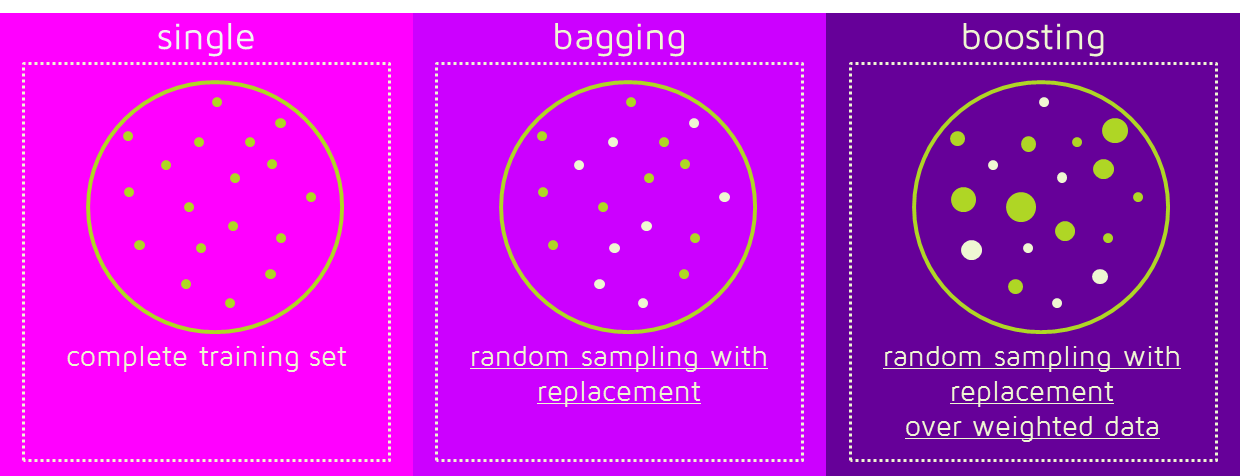
\includegraphics{figuras/bagging-boosting-1.png}
\caption{Bagging vs Boosting}
\end{figure}

    \hypertarget{bagging-vs-boosting-sequencial-vs-paralelo}{%
\section{Bagging vs Boosting: Sequencial vs
Paralelo}\label{bagging-vs-boosting-sequencial-vs-paralelo}}

\begin{figure}
\centering
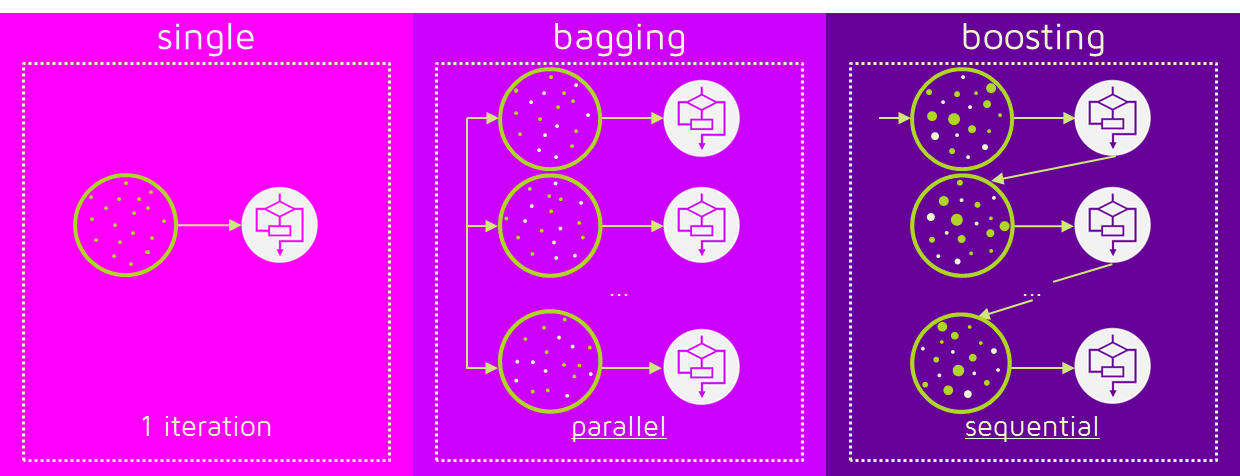
\includegraphics{figuras/bagging-boosting-2.png}
\caption{Bagging vs Boosting}
\end{figure}

    \hypertarget{bagging-vs-boosting-treinamento}{%
\section{Bagging vs Boosting:
Treinamento}\label{bagging-vs-boosting-treinamento}}

\begin{figure}
\centering
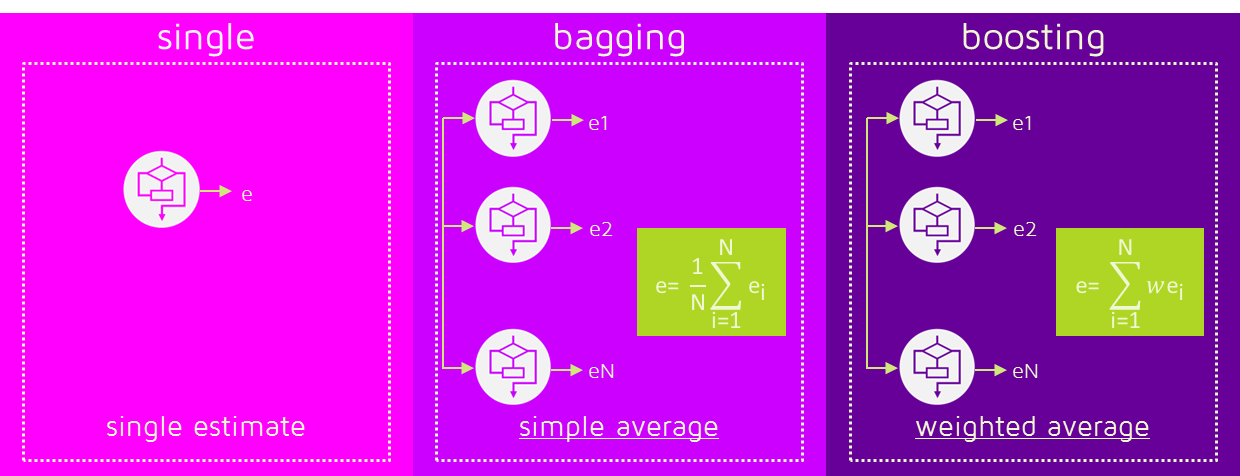
\includegraphics{figuras/bagging-boosting-3.png}
\caption{Bagging vs Boosting}
\end{figure}

    \hypertarget{bagging-vs-boosting-qual-uxe9-o-melhor}{%
\section{Bagging vs Boosting: qual é o
melhor?}\label{bagging-vs-boosting-qual-uxe9-o-melhor}}

Não há um vencedor: depende dos dados, da complexidade do problema e do
algoritmo base

Bagging e Boosting reduzem a variância de uma estimativa única. Modelo
com maior estabilidade.

Bagging raramente irá melhorar o viés de um modelo único com baixo
desempenho. Entretanto pode gerar um modelo combinado com menores erros.

Se o problema do modelo único é o overfitting, então Bagging é a melhor
opção. Boosting não ajuda a evitar/melhorar o overfitting.

    \hypertarget{stacking}{%
\section{Stacking}\label{stacking}}

Stacking é uma técnica de aprendizado por ensemble que combina múltiplos
modelos de classificação ou regressão através de um meta classificador
ou meta regressor.

Os modelos de base são treinados em um conjunto completo da base de
treinamento, e então o meta modelo utiliza as saídas dos modelos de base
como características de entrada.

A base geralmente utiliza diferentes algoritmos de aprendizado e
portanto geralmente stacking se refere a um modelo heterogêneos de
ensemble

    \hypertarget{stacking}{%
\section{Stacking}\label{stacking}}

\begin{figure}
\centering
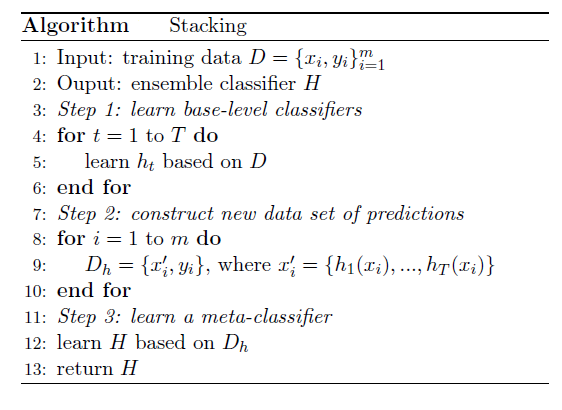
\includegraphics{figuras/stacking.png}
\caption{Stacking}
\end{figure}

    \hypertarget{stacking-exemplo}{%
\section{Stacking: Exemplo}\label{stacking-exemplo}}

    \begin{Verbatim}[commandchars=\\\{\}]
{\color{incolor}In [{\color{incolor}25}]:} \PY{k+kn}{import} \PY{n+nn}{itertools}
         \PY{k+kn}{import} \PY{n+nn}{numpy} \PY{k}{as} \PY{n+nn}{np}
         \PY{k+kn}{import} \PY{n+nn}{seaborn} \PY{k}{as} \PY{n+nn}{sns}
         \PY{k+kn}{import} \PY{n+nn}{matplotlib}\PY{n+nn}{.}\PY{n+nn}{pyplot} \PY{k}{as} \PY{n+nn}{plt}
         \PY{k+kn}{import} \PY{n+nn}{matplotlib}\PY{n+nn}{.}\PY{n+nn}{gridspec} \PY{k}{as} \PY{n+nn}{gridspec}
         
         \PY{k+kn}{from} \PY{n+nn}{sklearn} \PY{k}{import} \PY{n}{datasets}
         
         \PY{k+kn}{from} \PY{n+nn}{sklearn}\PY{n+nn}{.}\PY{n+nn}{linear\PYZus{}model} \PY{k}{import} \PY{n}{LogisticRegression}
         \PY{k+kn}{from} \PY{n+nn}{sklearn}\PY{n+nn}{.}\PY{n+nn}{naive\PYZus{}bayes} \PY{k}{import} \PY{n}{GaussianNB} 
         \PY{k+kn}{from} \PY{n+nn}{sklearn}\PY{n+nn}{.}\PY{n+nn}{ensemble} \PY{k}{import} \PY{n}{RandomForestClassifier}
         \PY{k+kn}{from} \PY{n+nn}{mlxtend}\PY{n+nn}{.}\PY{n+nn}{classifier} \PY{k}{import} \PY{n}{StackingClassifier}
\end{Verbatim}


    \begin{Verbatim}[commandchars=\\\{\}]
{\color{incolor}In [{\color{incolor}26}]:} \PY{n}{iris} \PY{o}{=} \PY{n}{datasets}\PY{o}{.}\PY{n}{load\PYZus{}iris}\PY{p}{(}\PY{p}{)}
         \PY{n}{X}\PY{p}{,} \PY{n}{y} \PY{o}{=} \PY{n}{iris}\PY{o}{.}\PY{n}{data}\PY{p}{[}\PY{p}{:}\PY{p}{,} \PY{l+m+mi}{1}\PY{p}{:}\PY{l+m+mi}{3}\PY{p}{]}\PY{p}{,} \PY{n}{iris}\PY{o}{.}\PY{n}{target}
         
         \PY{n}{clf1} \PY{o}{=} \PY{n}{KNeighborsClassifier}\PY{p}{(}\PY{n}{n\PYZus{}neighbors}\PY{o}{=}\PY{l+m+mi}{1}\PY{p}{)}
         \PY{n}{clf2} \PY{o}{=} \PY{n}{RandomForestClassifier}\PY{p}{(}\PY{n}{random\PYZus{}state}\PY{o}{=}\PY{l+m+mi}{1}\PY{p}{)}
         \PY{n}{clf3} \PY{o}{=} \PY{n}{GaussianNB}\PY{p}{(}\PY{p}{)}
         \PY{n}{lr} \PY{o}{=} \PY{n}{LogisticRegression}\PY{p}{(}\PY{p}{)}
         \PY{n}{sclf} \PY{o}{=} \PY{n}{StackingClassifier}\PY{p}{(}\PY{n}{classifiers}\PY{o}{=}\PY{p}{[}\PY{n}{clf1}\PY{p}{,} \PY{n}{clf2}\PY{p}{,} \PY{n}{clf3}\PY{p}{]}\PY{p}{,} 
                                   \PY{n}{meta\PYZus{}classifier}\PY{o}{=}\PY{n}{lr}\PY{p}{)}
\end{Verbatim}


    \begin{Verbatim}[commandchars=\\\{\}]
{\color{incolor}In [{\color{incolor}27}]:} \PY{n}{label} \PY{o}{=} \PY{p}{[}\PY{l+s+s1}{\PYZsq{}}\PY{l+s+s1}{KNN}\PY{l+s+s1}{\PYZsq{}}\PY{p}{,} \PY{l+s+s1}{\PYZsq{}}\PY{l+s+s1}{Random Forest}\PY{l+s+s1}{\PYZsq{}}\PY{p}{,} \PY{l+s+s1}{\PYZsq{}}\PY{l+s+s1}{Naive Bayes}\PY{l+s+s1}{\PYZsq{}}\PY{p}{,} \PY{l+s+s1}{\PYZsq{}}\PY{l+s+s1}{Stacking Classifier}\PY{l+s+s1}{\PYZsq{}}\PY{p}{]}
         \PY{n}{clf\PYZus{}list} \PY{o}{=} \PY{p}{[}\PY{n}{clf1}\PY{p}{,} \PY{n}{clf2}\PY{p}{,} \PY{n}{clf3}\PY{p}{,} \PY{n}{sclf}\PY{p}{]}
             
         \PY{n}{fig} \PY{o}{=} \PY{n}{plt}\PY{o}{.}\PY{n}{figure}\PY{p}{(}\PY{n}{figsize}\PY{o}{=}\PY{p}{(}\PY{l+m+mi}{10}\PY{p}{,}\PY{l+m+mi}{8}\PY{p}{)}\PY{p}{)}
         \PY{n}{gs} \PY{o}{=} \PY{n}{gridspec}\PY{o}{.}\PY{n}{GridSpec}\PY{p}{(}\PY{l+m+mi}{2}\PY{p}{,} \PY{l+m+mi}{2}\PY{p}{)}
         \PY{n}{grid} \PY{o}{=} \PY{n}{itertools}\PY{o}{.}\PY{n}{product}\PY{p}{(}\PY{p}{[}\PY{l+m+mi}{0}\PY{p}{,}\PY{l+m+mi}{1}\PY{p}{]}\PY{p}{,}\PY{n}{repeat}\PY{o}{=}\PY{l+m+mi}{2}\PY{p}{)}
         
         \PY{n}{clf\PYZus{}cv\PYZus{}mean} \PY{o}{=} \PY{p}{[}\PY{p}{]}
         \PY{n}{clf\PYZus{}cv\PYZus{}std} \PY{o}{=} \PY{p}{[}\PY{p}{]}
         \PY{k}{for} \PY{n}{clf}\PY{p}{,} \PY{n}{label}\PY{p}{,} \PY{n}{grd} \PY{o+ow}{in} \PY{n+nb}{zip}\PY{p}{(}\PY{n}{clf\PYZus{}list}\PY{p}{,} \PY{n}{label}\PY{p}{,} \PY{n}{grid}\PY{p}{)}\PY{p}{:}
                 
             \PY{n}{scores} \PY{o}{=} \PY{n}{cross\PYZus{}val\PYZus{}score}\PY{p}{(}\PY{n}{clf}\PY{p}{,} \PY{n}{X}\PY{p}{,} \PY{n}{y}\PY{p}{,} \PY{n}{cv}\PY{o}{=}\PY{l+m+mi}{3}\PY{p}{,} \PY{n}{scoring}\PY{o}{=}\PY{l+s+s1}{\PYZsq{}}\PY{l+s+s1}{accuracy}\PY{l+s+s1}{\PYZsq{}}\PY{p}{)}
             \PY{n+nb}{print}\PY{p}{(}\PY{l+s+s2}{\PYZdq{}}\PY{l+s+s2}{Accuracy: }\PY{l+s+si}{\PYZpc{}.2f}\PY{l+s+s2}{ (+/\PYZhy{} }\PY{l+s+si}{\PYZpc{}.2f}\PY{l+s+s2}{) [}\PY{l+s+si}{\PYZpc{}s}\PY{l+s+s2}{]}\PY{l+s+s2}{\PYZdq{}} \PY{o}{\PYZpc{}}\PY{p}{(}\PY{n}{scores}\PY{o}{.}\PY{n}{mean}\PY{p}{(}\PY{p}{)}\PY{p}{,} \PY{n}{scores}\PY{o}{.}\PY{n}{std}\PY{p}{(}\PY{p}{)}\PY{p}{,} \PY{n}{label}\PY{p}{)}\PY{p}{)}
             \PY{n}{clf\PYZus{}cv\PYZus{}mean}\PY{o}{.}\PY{n}{append}\PY{p}{(}\PY{n}{scores}\PY{o}{.}\PY{n}{mean}\PY{p}{(}\PY{p}{)}\PY{p}{)}
             \PY{n}{clf\PYZus{}cv\PYZus{}std}\PY{o}{.}\PY{n}{append}\PY{p}{(}\PY{n}{scores}\PY{o}{.}\PY{n}{std}\PY{p}{(}\PY{p}{)}\PY{p}{)}
                 
             \PY{n}{clf}\PY{o}{.}\PY{n}{fit}\PY{p}{(}\PY{n}{X}\PY{p}{,} \PY{n}{y}\PY{p}{)}
             \PY{n}{ax} \PY{o}{=} \PY{n}{plt}\PY{o}{.}\PY{n}{subplot}\PY{p}{(}\PY{n}{gs}\PY{p}{[}\PY{n}{grd}\PY{p}{[}\PY{l+m+mi}{0}\PY{p}{]}\PY{p}{,} \PY{n}{grd}\PY{p}{[}\PY{l+m+mi}{1}\PY{p}{]}\PY{p}{]}\PY{p}{)}
             \PY{n}{fig} \PY{o}{=} \PY{n}{plot\PYZus{}decision\PYZus{}regions}\PY{p}{(}\PY{n}{X}\PY{o}{=}\PY{n}{X}\PY{p}{,} \PY{n}{y}\PY{o}{=}\PY{n}{y}\PY{p}{,} \PY{n}{clf}\PY{o}{=}\PY{n}{clf}\PY{p}{)}
             \PY{n}{plt}\PY{o}{.}\PY{n}{title}\PY{p}{(}\PY{n}{label}\PY{p}{)}
\end{Verbatim}


    \begin{Verbatim}[commandchars=\\\{\}]
Accuracy: 0.91 (+/- 0.01) [KNN]
Accuracy: 0.91 (+/- 0.06) [Random Forest]
Accuracy: 0.92 (+/- 0.03) [Naive Bayes]
Accuracy: 0.95 (+/- 0.03) [Stacking Classifier]

    \end{Verbatim}

    \begin{Verbatim}[commandchars=\\\{\}]
{\color{incolor}In [{\color{incolor}28}]:} \PY{n}{plt}\PY{o}{.}\PY{n}{show}\PY{p}{(}\PY{p}{)}
\end{Verbatim}


    \begin{center}
    \adjustimage{max size={0.9\linewidth}{0.9\paperheight}}{output_49_0.png}
    \end{center}
    { \hspace*{\fill} \\}
    
    \begin{Verbatim}[commandchars=\\\{\}]
{\color{incolor}In [{\color{incolor}29}]:}    \PY{n}{plt}\PY{o}{.}\PY{n}{figure}\PY{p}{(}\PY{p}{)}
         \PY{p}{(}\PY{n}{\PYZus{}}\PY{p}{,} \PY{n}{caps}\PY{p}{,} \PY{n}{\PYZus{}}\PY{p}{)} \PY{o}{=} \PY{n}{plt}\PY{o}{.}\PY{n}{errorbar}\PY{p}{(}\PY{n+nb}{range}\PY{p}{(}\PY{l+m+mi}{4}\PY{p}{)}\PY{p}{,} \PY{n}{clf\PYZus{}cv\PYZus{}mean}\PY{p}{,} \PY{n}{yerr}\PY{o}{=}\PY{n}{clf\PYZus{}cv\PYZus{}std}\PY{p}{,} \PY{n}{c}\PY{o}{=}\PY{l+s+s1}{\PYZsq{}}\PY{l+s+s1}{blue}\PY{l+s+s1}{\PYZsq{}}\PY{p}{,} \PY{n}{fmt}\PY{o}{=}\PY{l+s+s1}{\PYZsq{}}\PY{l+s+s1}{\PYZhy{}o}\PY{l+s+s1}{\PYZsq{}}\PY{p}{,} \PY{n}{capsize}\PY{o}{=}\PY{l+m+mi}{5}\PY{p}{)}
         \PY{k}{for} \PY{n}{cap} \PY{o+ow}{in} \PY{n}{caps}\PY{p}{:}
             \PY{n}{cap}\PY{o}{.}\PY{n}{set\PYZus{}markeredgewidth}\PY{p}{(}\PY{l+m+mi}{1}\PY{p}{)}                                                                                                                                
         \PY{n}{plt}\PY{o}{.}\PY{n}{xticks}\PY{p}{(}\PY{n+nb}{range}\PY{p}{(}\PY{l+m+mi}{4}\PY{p}{)}\PY{p}{,} \PY{p}{[}\PY{l+s+s1}{\PYZsq{}}\PY{l+s+s1}{KNN}\PY{l+s+s1}{\PYZsq{}}\PY{p}{,} \PY{l+s+s1}{\PYZsq{}}\PY{l+s+s1}{RF}\PY{l+s+s1}{\PYZsq{}}\PY{p}{,} \PY{l+s+s1}{\PYZsq{}}\PY{l+s+s1}{NB}\PY{l+s+s1}{\PYZsq{}}\PY{p}{,} \PY{l+s+s1}{\PYZsq{}}\PY{l+s+s1}{Stacking}\PY{l+s+s1}{\PYZsq{}}\PY{p}{]}\PY{p}{)}        
         \PY{n}{plt}\PY{o}{.}\PY{n}{ylabel}\PY{p}{(}\PY{l+s+s1}{\PYZsq{}}\PY{l+s+s1}{Accuracy}\PY{l+s+s1}{\PYZsq{}}\PY{p}{)}\PY{p}{;} \PY{n}{plt}\PY{o}{.}\PY{n}{xlabel}\PY{p}{(}\PY{l+s+s1}{\PYZsq{}}\PY{l+s+s1}{Classifier}\PY{l+s+s1}{\PYZsq{}}\PY{p}{)}\PY{p}{;} \PY{n}{plt}\PY{o}{.}\PY{n}{title}\PY{p}{(}\PY{l+s+s1}{\PYZsq{}}\PY{l+s+s1}{Stacking Ensemble}\PY{l+s+s1}{\PYZsq{}}\PY{p}{)}\PY{p}{;}
         \PY{n}{plt}\PY{o}{.}\PY{n}{show}\PY{p}{(}\PY{p}{)}
\end{Verbatim}


    \begin{center}
    \adjustimage{max size={0.9\linewidth}{0.9\paperheight}}{output_50_0.png}
    \end{center}
    { \hspace*{\fill} \\}
    
    \begin{Verbatim}[commandchars=\\\{\}]
{\color{incolor}In [{\color{incolor}30}]:} \PY{n}{X\PYZus{}train}\PY{p}{,} \PY{n}{X\PYZus{}test}\PY{p}{,} \PY{n}{y\PYZus{}train}\PY{p}{,} \PY{n}{y\PYZus{}test} \PY{o}{=} \PY{n}{train\PYZus{}test\PYZus{}split}\PY{p}{(}\PY{n}{X}\PY{p}{,} \PY{n}{y}\PY{p}{,} \PY{n}{test\PYZus{}size}\PY{o}{=}\PY{l+m+mf}{0.3}\PY{p}{,} \PY{n}{random\PYZus{}state}\PY{o}{=}\PY{l+m+mi}{42}\PY{p}{)}
             
         \PY{n}{plt}\PY{o}{.}\PY{n}{figure}\PY{p}{(}\PY{p}{)}
         \PY{n}{plot\PYZus{}learning\PYZus{}curves}\PY{p}{(}\PY{n}{X\PYZus{}train}\PY{p}{,} \PY{n}{y\PYZus{}train}\PY{p}{,} \PY{n}{X\PYZus{}test}\PY{p}{,} \PY{n}{y\PYZus{}test}\PY{p}{,} \PY{n}{sclf}\PY{p}{,} \PY{n}{print\PYZus{}model}\PY{o}{=}\PY{k+kc}{False}\PY{p}{,} \PY{n}{style}\PY{o}{=}\PY{l+s+s1}{\PYZsq{}}\PY{l+s+s1}{ggplot}\PY{l+s+s1}{\PYZsq{}}\PY{p}{)}
         \PY{n}{plt}\PY{o}{.}\PY{n}{show}\PY{p}{(}\PY{p}{)}
\end{Verbatim}


    \begin{center}
    \adjustimage{max size={0.9\linewidth}{0.9\paperheight}}{output_51_0.png}
    \end{center}
    { \hspace*{\fill} \\}
    

    % Add a bibliography block to the postdoc
    
    
    
    \end{document}
